\documentclass[pdflatex,sn-basic]{sn-jnl}

\usepackage{graphicx}%
\usepackage{multirow}%
\usepackage{amsmath,amssymb,amsfonts}%
\usepackage{amsthm}%
\usepackage{mathrsfs}%
\usepackage[title]{appendix}%
\usepackage{xcolor}%
\usepackage{textcomp}%
\usepackage{manyfoot}%
\usepackage{booktabs}%
\usepackage{array}%
% ORCID iD after an author's name, as a link to the record
\newcommand{\orcidid}[1]{\href{https://orcid.org/#1}{\textsuperscript{\sffamily\bfseries\textcolor[HTML]{A6CE39}{iD}}}}%
\usepackage{tabularx}%
% floats are never set above the text that introduces them
\usepackage{flafter}%
% figures and tables are set in the text flow, right after the paragraph that introduces them
\makeatletter\providecommand\captionof[1]{\def\@captype{#1}\caption}\makeatother

\graphicspath{{figures/}}
\raggedbottom

% breakurl works only with pdflatex; other engines set reference URLs with \url
\usepackage{iftex}
\ifPDFTeX\else\AtBeginDocument{\let\burl\url}\fi
\hypersetup{pdftitle={Additional file 1. Supplementary material for ``Drift Detection, Diagnosis and Reliability Analysis for Deployed Machine Learning Models''}, pdfauthor={Rahul Guhagarkar, Nathan Cherian, Alok Pal, Akul Patre, Sanjay Mirchandani}}

\begin{document}

\title[Additional file 1. Supplementary material for ``Drift Detection, Diagnosis and Reliability Analysis for Deployed Machine Learning Models'']{Additional file 1. Supplementary material for ``Drift Detection, Diagnosis and Reliability Analysis for Deployed Machine Learning Models''}

\author*[1]{\fnm{Rahul} \sur{Guhagarkar}}\email{2023.rahul.guhagarkar@ves.ac.in}
\author[1]{\fnm{Nathan} \sur{Cherian}}
\author[1]{\fnm{Alok} \sur{Pal}}
\author[1]{\fnm{Akul} \sur{Patre}}
\author[1]{\fnm{Sanjay} \sur{Mirchandani}}

\affil*[1]{\orgdiv{Department of Computer Engineering}, \orgname{Vivekanand Education Society's Institute of Technology}, \orgaddress{\street{Hashu Advani Memorial Complex, Collector's Colony, Chembur}, \city{Mumbai}, \postcode{400074}, \country{India}}}



\maketitle

\noindent\emph{Section, figure, table and equation numbers without the prefix S refer to the main paper.}

\renewcommand{\thesection}{S\arabic{section}}
\renewcommand{\thefigure}{S\arabic{figure}}
\renewcommand{\thetable}{S\arabic{table}}
\renewcommand{\theequation}{S\arabic{equation}}

Five topics that the main paper only touches on are expanded here. Section~\ref{sec:budget} asks how many delayed labels the audit needs before its diagnosis settles. Section~\ref{sec:remediation} breaks the remediation triage down by real setting, while Section~\ref{sec:relp} records how the relationship codes of the American Community Survey (ACS) were matched across their 2019 redesign. Section~\ref{sec:dashboard} presents the dashboard in which the pipeline displays its results. The last section, Section~\ref{sec:seeds}, shows how the benchmark results vary over seeds and states.

\section{Size of the delayed audit}\label{sec:budget}

The audit stage of Section~2.1.3 needs late labels. Labels cost money, so it matters how many are enough. The paper uses 600 labels throughout. Fig.~\ref{fig:budget} shows how the share of correctly diagnosed windows changes with the size of the audit on ACS Income design A with logistic regression (LR).

\begin{figure}[!htbp]\centering
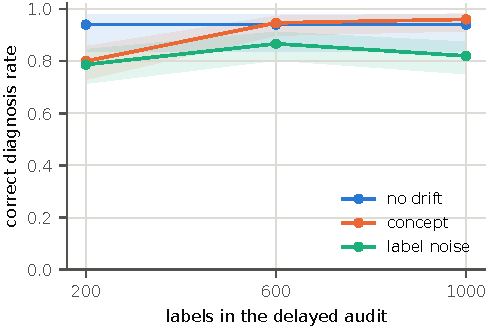
\includegraphics[width=83.5mm,height=0.6\textheight,keepaspectratio]{FigS1.pdf}
\caption{Share of correctly diagnosed windows on ACS Income design A with LR against the number of audit labels. The shaded bands are 95\% Wilson intervals}\label{fig:budget}
\end{figure}

With 200 labels, concept drift is identified in 80\% of windows and label noise in 79\%. With 600 labels the two rates reach 95\% and 87\%. Going on to 1000 labels adds little (96\% and 82\%). The 600 labels of the paper therefore sit where more labels stop paying off. The control windows are diagnosed correctly in the same share of cases at every audit size.


\section{Remediation triage by setting}\label{sec:remediation}

Section~3.5 of the paper summarizes how often the triage of Section~2.1.5 gives the right advice. Table~\ref{tab:remediation} breaks this summary down by real setting and model family, so that the source of each right or wrong verdict can be seen.

\begin{table}[!htbp]\centering\tablebodyfont
\caption{Remediation triage on the real windows. n is the number of windows; Significant gains counts the windows in which a strategy significantly raised holdout accuracy, by importance weighting (IW), retraining on the most recent labeled window (Recent) or retraining on labels of the window itself (Labels); n/a marks settings without an earlier window}\label{tab:remediation}%
\setlength{\tabcolsep}{4pt}
\begin{tabularx}{\textwidth}{@{}l>{\raggedright\arraybackslash}Xrrrrrrrr@{}}
\toprule
 &  & \multicolumn{1}{c}{} & \multicolumn{3}{c}{Significant gains} & \multicolumn{3}{c}{Triage} & \multicolumn{1}{c}{Rule} \\
\cmidrule(lr){4-6}
\cmidrule(lr){7-9}
\cmidrule(lr){10-10}
Model & Settings & \multicolumn{1}{c}{$n$} & \multicolumn{1}{c}{IW} & \multicolumn{1}{c}{Recent} & \multicolumn{1}{c}{Labels} & \multicolumn{1}{c}{Escalated} & \multicolumn{1}{c}{\begin{tabular}[b]{@{}c@{}}Truly\\ helps\end{tabular}} & \multicolumn{1}{c}{Correct} & \multicolumn{1}{c}{Correct} \\
\midrule
LR & ACS Income, temporal & 8 & 4/8 & 7/7 & 5/8 & 7 & 7 & 8/8 & 8/8 \\
 & ACS Income, states & 4 & 0/4 & n/a & 4/4 & 0 & 0 & 4/4 & 4/4 \\
 & ACS Employment, temporal & 8 & 4/8 & 7/7 & 2/8 & 7 & 7 & 8/8 & 8/8 \\
 & ACS Employment, states & 4 & 2/4 & n/a & 1/4 & 1 & 2 & 3/4 & 2/4 \\
 & CLEAR-10 & 9 & 0/9 & 4/8 & 6/9 & 4 & 4 & 7/9 & 5/9 \\
 & Gas sensor & 8 & 1/8 & 7/7 & 8/8 & 7 & 7 & 8/8 & 8/8 \\
\midrule
GB & ACS Income, temporal & 8 & 0/8 & 7/7 & 4/8 & 7 & 7 & 8/8 & 8/8 \\
 & ACS Income, states & 4 & 0/4 & n/a & 3/4 & 0 & 0 & 4/4 & 4/4 \\
 & ACS Employment, temporal & 8 & 0/8 & 7/7 & 0/8 & 6 & 7 & 7/8 & 8/8 \\
 & ACS Employment, states & 4 & 0/4 & n/a & 0/4 & 0 & 0 & 4/4 & 4/4 \\
 & CLEAR-10 & 9 & 0/9 & 8/8 & 9/9 & 8 & 8 & 9/9 & 9/9 \\
 & Gas sensor & 8 & 1/8 & 5/7 & 8/8 & 7 & 6 & 7/8 & 7/8 \\
\botrule
\end{tabularx}
\footnotetext{Escalated counts the windows in which the triage recommended a retrain, Truly helps those in which a cheap retrain did help and Correct the windows in which the advice was right. Rule counts the windows in which the simple rule of retraining exactly when an earlier labeled window exists was right}
\end{table}

Where an earlier labeled window exists, retraining on it helps in almost every temporal window. The triage escalates in those windows. The geographic windows of the census tasks have no earlier window. There, importance weighting rarely helps and the triage mostly advises against a retrain. Most of the remaining wrong verdicts come from CLEAR-10 with LR and from the geographic windows of ACS Employment. The simple rule in the last column is right about as often as the triage, which is why the paper reports the triage as a negative result.

\section{Relationship codes across the 2019 redesign}\label{sec:relp}

The ACS windows run from 2014 to 2023, but one of their features changed its coding halfway through. From 2019 the Census Bureau replaced the relationship variable RELP with RELSHIPP, whose codes split spouses and partners by sex~\citep{census2019pums}. To compare windows before and after 2019, we map the RELSHIPP codes back to RELP by matching the code labels of the 2018 and 2019 data dictionaries. Table~\ref{tab:relp} lists the mapping as the code applies it.

\begin{table}[!htbp]\centering\tablebodyfont
\caption{Mapping from RELSHIPP (2019 on) back to RELP (2014 to 2018)}\label{tab:relp}%
\begin{tabular}{@{}rll@{}}
\toprule
RELP & Label (2018) & RELSHIPP codes (2019 on) \\
\midrule
0 & Reference person & 20 \\
1 & Husband/wife & 21, 23 \\
2 & Biological son or daughter & 25 \\
3 & Adopted son or daughter & 26 \\
4 & Stepson or stepdaughter & 27 \\
5 & Brother or sister & 28 \\
6 & Father or mother & 29 \\
7 & Grandchild & 30 \\
8 & Parent-in-law & 31 \\
9 & Son-in-law or daughter-in-law & 32 \\
10 & Other relative & 33 \\
11 & Roomer or boarder & none \\
12 & Housemate or roommate & 34 \\
13 & Unmarried partner & 22, 24 \\
14 & Foster child & 35 \\
15 & Other nonrelative & 36 \\
16 & Institutionalized group quarters population & 37 \\
17 & Noninstitutionalized group quarters population & 38 \\
\botrule
\end{tabular}
\end{table}

RELP 11 (roomer or boarder) has no successor, so it never occurs from 2019 on. The loss of this category is itself a documented change that the localization can pick up.


\section{The monitoring dashboard}\label{sec:dashboard}

A diagnosis is only useful if the team can read it. Every stage of the pipeline therefore writes its results to one file, which an interactive dashboard presents. Fig.~\ref{fig:dashboard} shows two of its views for ACS Income with LR.

\begin{figure}[!htbp]\centering
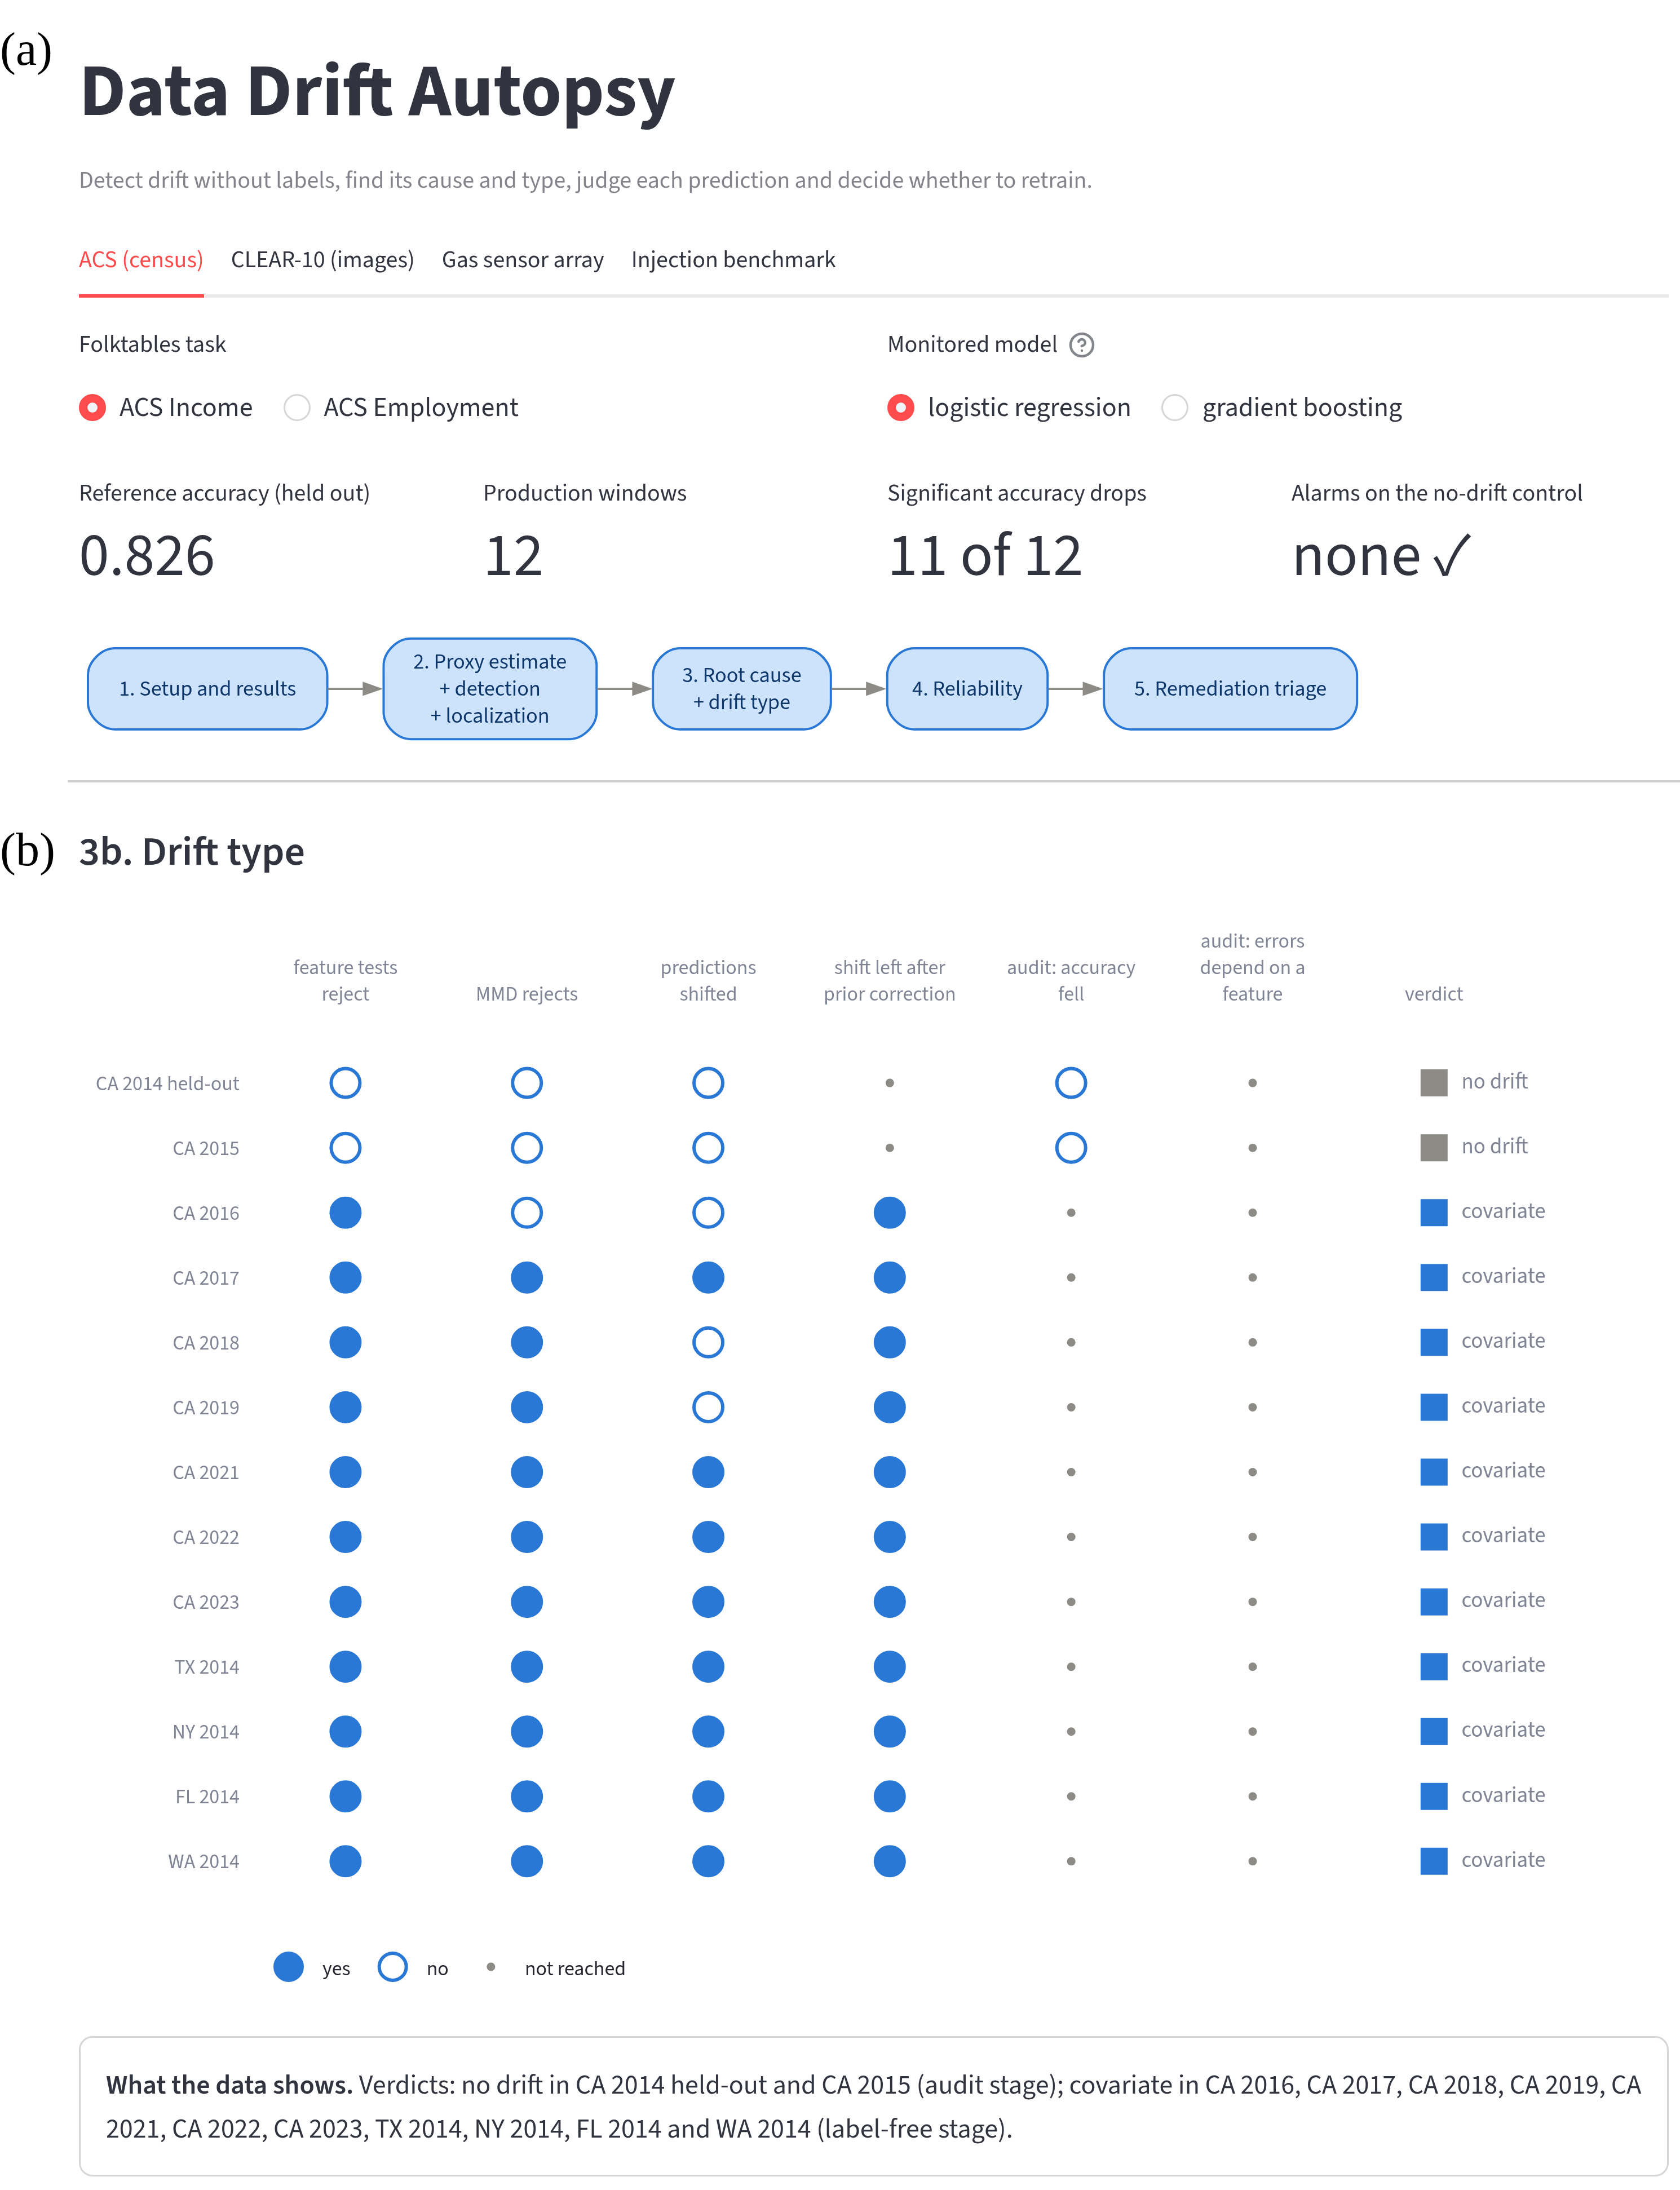
\includegraphics[width=\textwidth,height=0.6\textheight,keepaspectratio]{FigS2.png}
\caption{The dashboard of the pipeline for ACS Income with LR. (a) The overview: dataset, task and model selectors, the headline results and the five steps of the pipeline, each of which opens a detailed view. (b) The drift type step: for every window, the answer to each question of the decision path in Fig.~2 of the paper (filled circle yes, open circle no, small dot not reached) and the resulting verdict, followed by a summary sentence computed from the results}\label{fig:dashboard}
\end{figure}

Panel (b) applies the decision path of Fig.~2 to the real California (CA) windows. CA 2015 passes every test of the label-free stage. The KS detector in Table~7 of the paper does raise an alarm on CA 2015, because it corrects only over the numeric features, while the label-free stage tests all features together with the other two blocks in one weighted Holm family (Section~2.1.3). The audit then finds no significant drop in accuracy, so the verdict is no drift. In CA 2016, CA 2018 and CA 2019 the predicted labels stay where they were. The feature tests still reject and the shift survives the prior correction, so these windows are covariate shift. All other windows answer yes to every label-free question and are covariate shift as well. Each view of the dashboard opens with the question it answers and closes with a summary sentence of this kind, so a team can follow the diagnosis without reading the code.

\section{Spread over seeds and states}\label{sec:seeds}

The shares in Tables~3 and 4 of the paper pool the windows of all five states and ten seeds. Table~\ref{tab:seedsmethods} shows how much the share of correctly typed windows varies and Table~\ref{tab:seedsmechanisms} does the same for the design B mechanisms. Each cell gives the mean and standard deviation of the share over the ten seeds, where each seed pools its five states. The interval in brackets treats the state as the cluster: it is a 95\% t interval with four degrees of freedom over the five state shares, cut at 0 and 100\%. Five clusters make these intervals wide.

\begin{table}[!htbp]\centering\tablebodyfont
\caption{Share of benchmark windows with the correct drift type over seeds and states (\%)}\label{tab:seedsmethods}%
\begin{tabular}{@{}llrrrr@{}}
\toprule
Model & Method & \multicolumn{1}{c}{Inc. A} & \multicolumn{1}{c}{Inc. B} & \multicolumn{1}{c}{Emp. A} & \multicolumn{1}{c}{Emp. B} \\
\midrule
LR & Ours (hierarchical tests) & 94.3 $\pm$ 7.6 & 62.4 $\pm$ 3.5 & 85.7 $\pm$ 5.6 & 80.5 $\pm$ 4.9 \\
 &  & [88, 100] & [59, 66] & [79, 92] & [77, 84] \\
 & Input monitoring & 30.3 $\pm$ 1.0 & 20.0 $\pm$ 0.0 & 30.6 $\pm$ 0.5 & 25.0 $\pm$ 0.0 \\
 &  & [30, 31] & [20, 20] & [30, 31] & [25, 25] \\
 & BBSE first & 30.5 $\pm$ 1.0 & 27.7 $\pm$ 5.4 & 30.5 $\pm$ 1.0 & 39.2 $\pm$ 9.7 \\
 &  & [30, 31] & [24, 31] & [30, 31] & [37, 42] \\
 & Error-rate monitoring & 52.3 $\pm$ 3.8 & 48.5 $\pm$ 6.8 & 52.2 $\pm$ 3.8 & 62.8 $\pm$ 10.7 \\
 &  & [50, 55] & [45, 53] & [50, 54] & [59, 66] \\
 & Learned meta-classifier & 97.4 $\pm$ 1.8 & 31.7 $\pm$ 3.1 & 95.7 $\pm$ 1.7 & 48.5 $\pm$ 7.1 \\
 &  & [96, 99] & [24, 39] & [94, 97] & [43, 54] \\
 & Ours without MMD block & 95.2 $\pm$ 4.9 & 62.9 $\pm$ 2.5 & 86.6 $\pm$ 4.0 & 81.3 $\pm$ 3.4 \\
 &  & [90, 100] & [59, 67] & [81, 92] & [77, 85] \\
 & Ours, audit null without confidence & 79.1 $\pm$ 5.2 & 62.9 $\pm$ 3.9 & 83.7 $\pm$ 5.4 & 80.7 $\pm$ 4.5 \\
 &  & [75, 83] & [58, 68] & [77, 90] & [77, 84] \\
 & Ours, audit null with class cells & 93.1 $\pm$ 8.0 & 65.6 $\pm$ 4.2 & 86.2 $\pm$ 6.7 & 91.8 $\pm$ 5.4 \\
 &  & [87, 99] & [61, 70] & [79, 93] & [89, 94] \\
\midrule
GB & Ours (hierarchical tests) & 94.2 $\pm$ 8.0 & 63.2 $\pm$ 3.6 & 90.5 $\pm$ 3.5 & 81.5 $\pm$ 3.5 \\
 &  & [88, 100] & [60, 66] & [84, 97] & [78, 85] \\
 & Input monitoring & 30.3 $\pm$ 1.0 & 20.0 $\pm$ 0.0 & 30.6 $\pm$ 0.5 & 25.0 $\pm$ 0.0 \\
 &  & [30, 31] & [20, 20] & [30, 31] & [25, 25] \\
 & BBSE first & 30.5 $\pm$ 1.0 & 28.1 $\pm$ 5.9 & 30.6 $\pm$ 0.5 & 40.3 $\pm$ 9.2 \\
 &  & [30, 31] & [25, 31] & [30, 31] & [38, 43] \\
 & Error-rate monitoring & 52.5 $\pm$ 3.9 & 49.6 $\pm$ 7.7 & 53.1 $\pm$ 2.0 & 64.8 $\pm$ 9.6 \\
 &  & [50, 55] & [46, 53] & [51, 55] & [62, 68] \\
 & Learned meta-classifier & 98.3 $\pm$ 1.7 & 39.2 $\pm$ 2.7 & 97.5 $\pm$ 2.4 & 50.7 $\pm$ 6.6 \\
 &  & [97, 100] & [37, 41] & [97, 98] & [46, 55] \\
 & Ours without MMD block & 95.1 $\pm$ 5.2 & 63.9 $\pm$ 2.2 & 90.5 $\pm$ 3.1 & 81.3 $\pm$ 4.4 \\
 &  & [89, 100] & [60, 68] & [84, 97] & [79, 83] \\
 & Ours, audit null without confidence & 78.0 $\pm$ 6.2 & 62.9 $\pm$ 3.3 & 85.4 $\pm$ 4.3 & 82.0 $\pm$ 3.2 \\
 &  & [75, 81] & [60, 66] & [80, 91] & [79, 85] \\
 & Ours, audit null with class cells & 92.9 $\pm$ 8.2 & 66.5 $\pm$ 4.2 & 90.6 $\pm$ 3.9 & 93.7 $\pm$ 4.4 \\
 &  & [86, 100] & [62, 71] & [84, 97] & [91, 96] \\
\botrule
\end{tabular}
\footnotetext{Inc. and Emp. stand for ACS Income and ACS Employment, A and B for the two designs}
\end{table}

\begin{table}[!htbp]\centering\tablebodyfont
\caption{Correct diagnosis by design B mechanism over seeds and states (\%)}\label{tab:seedsmechanisms}%
\begin{tabular}{@{}lrrrr@{}}
\toprule
 & \multicolumn{2}{c}{ACS Income} & \multicolumn{2}{c}{ACS Employment} \\
\cmidrule(lr){2-3}
\cmidrule(lr){4-5}
Mechanism & \multicolumn{1}{c}{LR} & \multicolumn{1}{c}{GB} & \multicolumn{1}{c}{LR} & \multicolumn{1}{c}{GB} \\
\midrule
Covariate: selection bias & 99.3 $\pm$ 2.1 & 99.3 $\pm$ 2.1 & 100.0 $\pm$ 0.0 & 100.0 $\pm$ 0.0 \\
 & [97, 100] & [97, 100] & [100, 100] & [100, 100] \\
Prior: decrease & 92.0 $\pm$ 9.3 & 92.7 $\pm$ 8.0 & 96.7 $\pm$ 6.5 & 96.7 $\pm$ 6.5 \\
 & [82, 100] & [84, 100] & [91, 100] & [91, 100] \\
Concept: oblique region & 95.3 $\pm$ 12.6 & 95.3 $\pm$ 12.6 & 90.7 $\pm$ 13.0 & 96.7 $\pm$ 6.5 \\
 & [89, 100] & [89, 100] & [81, 100] & [92, 100] \\
Concept: income threshold & 4.0 $\pm$ 4.7 & 6.0 $\pm$ 5.8 & -- & -- \\
 & [0, 9] & [0, 12] &  &  \\
Noise: class-conditional & 21.3 $\pm$ 8.2 & 22.7 $\pm$ 7.2 & 34.7 $\pm$ 11.7 & 32.7 $\pm$ 9.1 \\
 & [13, 30] & [14, 32] & [24, 45] & [25, 41] \\
\botrule
\end{tabular}
\end{table}

\bibliography{references}

\end{document}
